\addcontentsline{toc}{subsubsection}{Active Directory Basics}
\subsubsection*{Active Directory Basics}
\T{Introduction}{
Active Directory is a key tool in order to manage users and devices, and in thsi room we will learn about it, what its Domains are and which components they have, about Forests and Domain Trust, among others. 
}
\T{Windows Domains}{
In order to administer a large(r) network, where manual login and configuration is unfeasible, IT administrators use a \textbf{Windows domain}. It consists of a group of users and computers under the same administration which can this way be centrally administered in a single repository, called \textbf{Active Directory}. The server running this Active Directory (AD) services is the \textbf{Domain Controller} (DC).\\
The main advantages of this administration form are the centralised identity and security policies management.\\
This way of administration is commonly found in school or university networks allowing a login via authentication at the Active Directory at any machine in the network.This way, no actual computer needs to store any set of credentials.\\

In the rest of this module, we will be posing as the IT admin of THM.Inc to review the domain ``THM.local''.
}
\T{Active Directory}{
The core of the Windows Domains is the\textbf{Active Directory Domain Service}, which serves as a catalogue of the existing items in the network, be it users, groups and other peripherals. \\
Category-wise, we distinguish:\\
\begin{itemize}
\item \textbf{Users:} part of the \textbf{security principals}, i.e eligible for the assignment of security provileges over other parts of the network, users conform one of the most basic object types in the AD.\\
Users can be further divided into People and Services, the latter used to define non-personal users upon which specific services run, e.g IIS or MSSQL. These users will always only have the minimum privileges required to run correctly.
\item \textbf{Machines:} these objects represent every computer joining the Active Directory domain on a 1-to-1 relation. They are also part of the aforementioned security principals and use accounts the same way a personal user does, nonetheless with limited privileges.\\
The machine account always acts as a local administrator on the computer it represents and can be accessed with the corresponding credentials, altough they are usually not meant to. The passwords for these machine accounts are rotated out automatically and are comprised of 120 random characters.\\
The naming scheme of machine accounts uses the following pattern: <Machine name>\$, hence a machine called MyLaptop will have the account name \cd{MyLaptop\$}
\item \textbf{Security Groups:} instead of assigning rights on an individualized user basis, one can define user groups to manage their rights as a bulk, increasing its speed an ease.\\
E.g, a user newly added to a group will immediately inherit all of said group's rights. \\
Security Groups are also part of the security principals. They can contain Users and Machines, as well as other groups.\\
The following groups are created by default in an Active Domain:
\begin{itemize}
\item Domain Admins: these users have admin privileges over the whole domain and can administer any resource, including the Domain Controllers (DCs)
\item Server Operators: these users can administer DCs, but not change administrative group memberships
\item Backup Operators: these users can access any file regardless of permissions and are used to back up data
\item Account Operators: these users can create or modify other accounts on the domain
\item Domain Users: all exisiting user accounts in the domain
\item Domain Computers: all existing computers in the domain
\item Domain Controllers: all existing DCs on the domain
\end{itemize}
Further information about the default security groups can be found on \href{https://docs.microsoft.com/en-us/windows/security/identity-protection/access-control/active-directory-security-groups}{this documentation}.
\end{itemize}

In order to manage the users, groups, machines and further resources in the Active Directory, we log into the Domain Controller and run ``Active Directory Users and Computers''.\\
After so doing, we will see the hierarchy of users, computers and groups in the domain, organized in \textbf{Organizational Units (OUs)}.\\
These OUs refer to container objects used to classify users and machines, used to define sets of users with similar privileges or policing requirements, e.g department-wise.\\
A user can only be part of one OU at a time.

In the deployed machine we see an already deployed OU with subdependent (or child) OUs: IT, Management, Marketing and Sales. \\
Commonly, the OU mimics the business structure to allow for a task-dependent management of permits, privileges and policies. This structure is not mandatory, though. \\
When opening any OU, the corresponding administrator can see the users under said Organizational Unit and eventually reset passwords if needed.

The default containers from the Windows OS are:
\begin{itemize}
\item \textbf{Builtin:} OU for default groups for any Windows host
\item \textbf{Computers:} default OU for machine accounts
\item \textbf{Domain Controllers:} default OU for DCs
\item \textbf{Users:} default OU for users and groups
\item \textbf{Managed Service Accounts:} default OU for service user accounts. 
\end{itemize}

The main difference between Organizational Units and Security Groups rely on their target:\\
Organizational Units are used to apply policies and configurations depending on their role within the network, as any user can only be in one OU at a time. \\
Security Groups are used to grant permissions and privileges over resources, as any user can belong to many different Security Groups, especially useful to allow finer granularity over the access(es).\\

This task's question are merely a reading comprehension of the text above:
\QA{
Which group normally administrates all computers and resources in a domain?
}{
Domain Admins
}
\QA{
What would be the name of the machine account associated with a machine named TOM-PC?
}{
Tom-PC\$
}
\QA{
Suppose our company creates a new department for Quality Assurance. What type of containers should we use to group all Quality Assurance users so that policies can be applied consistently to them?
}{
Organizational Unit
}
}
\T{Managing Users in AD}{
In the deployed machine, we will have to structure the Active Directory corresponding to the following organisational chart:\\
\begin{center}
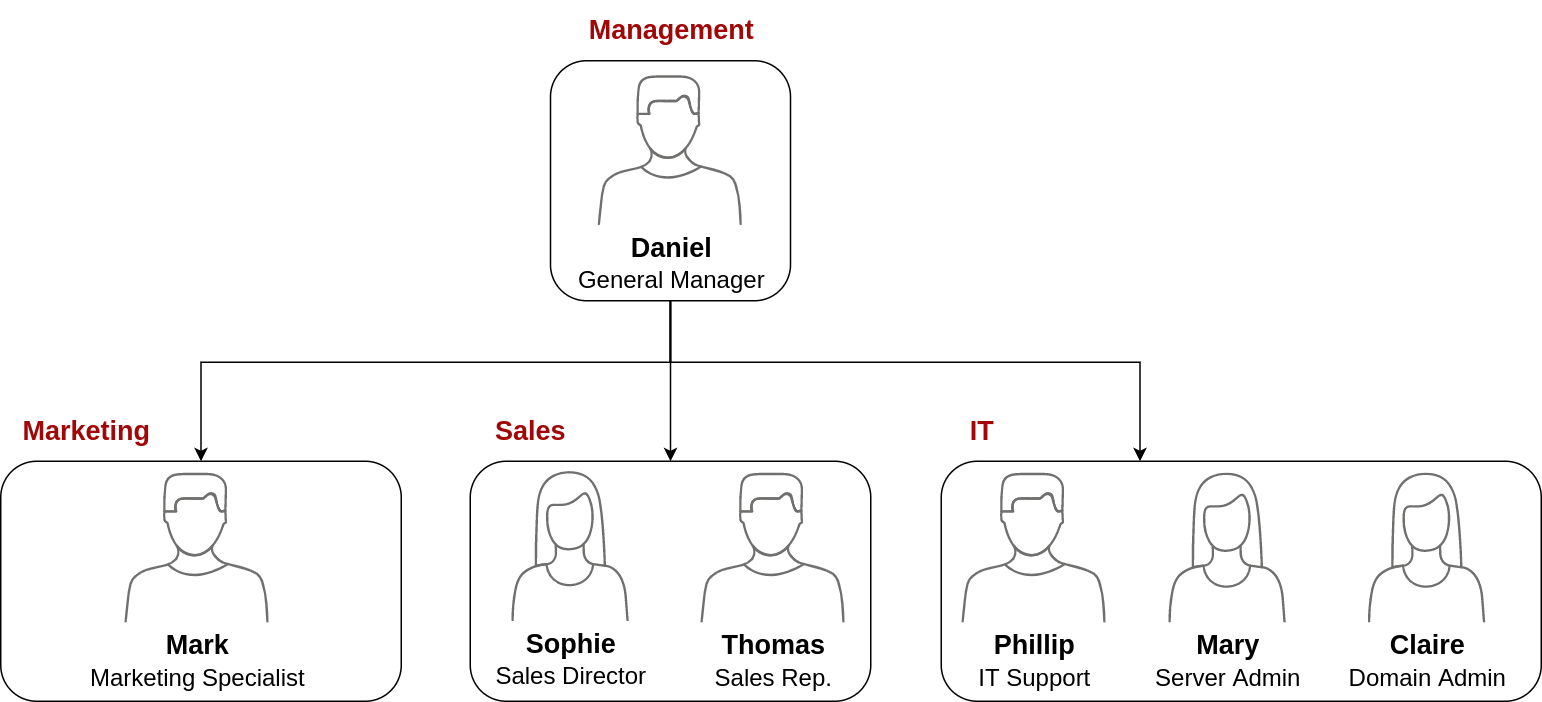
\includegraphics[scale=0.2]{Complete_Beginner_Path/Windows_Exploitation_Basics_Room/chart_AD_THM.png}
\end{center}
In order to do so, we have to first delete the department ``Research and Development''.\\
Our first attempt fails, as the group is prevented from accidental deletion. In order to be able to do so, we first have to enable the andvanced properties under ``View > Advanced Properties''. After being sent to the start chart and accessing the THM Active Directory again, we can right-click the corresponding OU and, under Properties, uncheck the ``Protect object from accidental deletion''-box.\\
Once this is done, we can proceed with the intended deletion of the OU and its dependent user, Bob.

We further need to adjust the users to match the chart above:\\we delete the ``Sales'' users Robert and Christine.\\

%Another useful tool from the Active Directory is the delegation of management or control. This is meant to give some privileged users the right to perform advanced tasks on OUs without the need for a Domain Administrator. This is most commonly the case for IT Support, as they might need to administer some lower privileged accounts, resetting passwords among other tasks. \\
In this example machine we will delegate the control of resetting passwords over all other departments to IT Support, consisting \textit{de facto} only of Phillip.\\
To perform this delegation, we go to the OU we want to delegate control of and then add the IT Support user (Phillip) to the users to whom we wish to delegate control to. As a note, we want to pay attention to the ``Check Names'' button in order to avoid misconfigurations and assign the delegation to the right user or group.\\
We then check the ``reset user passwords and force password change at next logon'' box and end the procedure.\\

Using RDP at the Computer given by the IP on the deployed machine and then providing the credentials from the task (phillip:Claire2008) we can run the commands given by the room to reset Sophie's password:

\cdnl{PS C:$\bsl$Users$\bsl$phillip> Set-ADAccountPassword sophie -Reset -NewPassword (Read-Host -AsSecureString -Prompt 'New Password') -Verbose}
we then provide the new password as instructed and see:
\cdnl{
VERBOSE: Performing the operation "Set-ADAccountPassword" on target "CN=Sophie,OU=Sales,OU=THM,DC=thm,DC=local"
}
In order to avoid us knowing Sophie's password, we then run the command to force her to change the password at logon:
\cdnl{PS C:$\bsl$Users$\bsl$phillip> Set-ADUser -ChangePasswordAtLogon \$true -Identity sophie -Verbose\\
VERBOSE: Performing the operation "Set" on target "CN=Sophie,OU=Sales,OU=THM,DC=thm,DC=local".
}
There, we see a text file containing the flag for this task:
\F{THM\{thanks\_for\_contacting\_support\}}
\QA{
The process of granting privileges to a user over some OU or other AD Object is called...
}{
Delegation
}
}
\T{Managing Computers in AD}{
By default, all machines joining a domain are added into the chart under the ``Computers'' container, as stated in the previous task.We can identify the kind of device in the domain by the abbreviation at the beginning of the name: ``SVR'' for servers, ``PC'' for PCs and ``LPT'' for laptops. \\
This indiscriminated list is not the best practice, nor the most useful, as we would like to assign different policies for servers and ``regular'' machines.\\
In general, it is a good idea to separate the machines on the domain according to use, commonly into the three following categories: 
\begin{itemize}
\item \textbf{Workstations:} one of the most common device kinds, this is the machine type a user logs into for their daily work usage. They shall not have a privileged user signed into them.
\item \textbf{Servers:} used to provide services to other elements in the domain such as users or other servers.
\item \textbf{Domain Controllers:} as seen before, DCs allow the administrators to manage the AD Domain. As such, they are the most sensitive devices, where hashed passwords are stored. 
\end{itemize}
On the deployed machine, we will separate the machines in Organizational Units according to their categories for the first two types, as DCs are already in a separate category per Windows default. \\
We first create the two separate OUs under THM.local ``Workstations'' and ``Servers''. After going back to ``Computers'', we select all three machines with name starting with SRV and under ``Move...'' place them in the newly created OU. We then do the same with the PCs and Laptops of the ``Computers'' OU, moving all seven to the ``Workstations'' OU.
\QA{
After organising the available computers, how many ended up in the Workstations OU?
}{
7
}
\QA{
Is it recommendable to create separate OUs for Servers and Workstations? (yay/nay)
}{
As implicitly stated in the text above under the ``good practice'' statement, we take it to be a positive recommendation, hence giving the answer \textbf{yay}.
}
}
\T{Group Policies}{
The whole point of creating and managing the previous Organizational Units was to assign tailored policies to every OU.\\
This can be done through Group Policy Objects (GPOs), a collection of settings to be applied to each user category, be it machines or users, and OUs. We can access said GPOs trhough the Group Policy Management tool.\\
There, we see the already known OU hierarchy as in previous tasks with the associated policies visible at dropdown. \\
We can create new GPOs under ``Group Policy Objects'' and later assign them to the OUs we want to link them to.\\
Note that GPOs preserve the hierarchichal structure, hence applying to every underlying OU to the one we assign them to.\\
In the deployed machine we see Default Domain Policy and RDP policy applying to every OU and ``Default Domain Controllers Policy'' applying to the Domain Controllers OU.\\

To get an idea of how GPOs look like, we analyze the Default Domain Policy and see the following organizational aspects in the tabs: 
\begin{itemize}
\item Scope: sets the application of the GPO and displays the eventual OUs it is linked to.\\
Here one can apply Security Filtering to GPOs to further restrict the scope. The default application is ``Authenticated Users'', which comprises all users and machines.
\item Settings: hierarchical report of the details of the GPO and its configuration, divided in ``General'', ``Computer Configuration'' and ``User Configuration'' in a ``tree-like'' representation. \\
To change the policies, we right-click on the corresponding Group Policy Object and under ``Edit'' we are free to adapt it to our needs.\\
We can read a description of each category under the editing menu on the left, and each terminal branch, i.e actual configuration setting, has an ``Explain'' tab for further clarification when needed.
\end{itemize}

GPOs are distributed to the network via a network share called \textbf{\cd{SYSVOL}}, stored in the Domain Controller, to which all users should have access to. Per default, it is located under \cd{C:$\bsl$Windows$\bsl$SYSVOL$\bsl$sysvol$\bsl$}.\\
The changes cantake some time to synchronize, so we can force the synchronization with the command\\
\cd{gpupdate /force} on the Powershell of the computer to be synchronized. 

In the context of the deployed machine, still within our fictive role as the IT admin of THM Inc., we will have to block non-IT users from accessing the Control Panel and make workstations and servers lock their screen automatically after 5 minutes of inactivity.\\

The first task can be completed by creating a GPO, preferrablly with a self explaining name such as ``Restrict Control Panel Access'' and adjusting its settings under ``User Configuration > Policies > Administrative Templates > Control Panel > Prohibit access to Control Panel and PC settings''. Once enabled, we only have to link it to the corresponding OUs either by right-clicking on them and linking the desired GPO or by dragging the GPO to the OU in the hierarchichal view to Marketing, Management and Sales.\\

For the second task, we can either create a GPO and apply it to every relevant object in the Active Directory, i.e Workstations, Servers and Domain Controllers, or apply it to the root domain which affects every child OU, which again affects every machine in the network.\\
Note that it will be inherited by other user OUs, but it does not matter as they only contain users.\\
The route to the AutoLock screen time is as follows:
``Policies > Windows Settings > Security Settings > Local Policies > Security Options > Interactive logon: Machine inactivity limit" and the time is measured in seconds.\\

We create this GPO, log in as Mark from Marketing with the given credentials and confirm the impossibilit to access the Control Panel, as desired. \\

\QA{
What is the name of the network share used to distribute GPOs to domain machines?
}{
SYSVOL
}
\QA{
Can a GPO be used to apply settings to users and computers? (yay/nay)
}{
yay
}
}
\T{Authentication Methods}{
Since we are dealing with user administration, some form of authentication is needed; in this case the credentials are checked against the stored credentials in the Domain Controller. There are two protocols in use for windows domains: \textbf{Kerberos}, the default protocol for modern versions, and \textbf{NetNTLM}, only kept for compatibility purposes with older domains. \\

When using Kerberos, any user will be assigned a ticket after logging in to be used later as a proof of previous authentication before the \textbf{Key Distribution Center (KDC)}, a service on the DC administering the Kerberos tickets on the network. This process takes place in the following way: 
\begin{enumerate}
\item The user sends the username and an encrypted timestamp using their password as encryption key to the KDC requesting a  \textbf{Ticket Generating Ticket (TGT)}.
\item The KDC creates and sends back an encrypted TGT, encoded with the KDC private key. \\
This ticket will allow the user to access other services after the corresponding ticket request without needing to pass the credentials every time.\\
Note that the TGT includes an encrypted copy of the (following) session key, hence allowing the Kerberos Distribution Center to ``forget'' the credentials o the user and only needing to recover their session key decrypting the TGT.
\item A Session Key is passed from the KDC to the Client, used to generate subsequent requests. 
\end{enumerate}
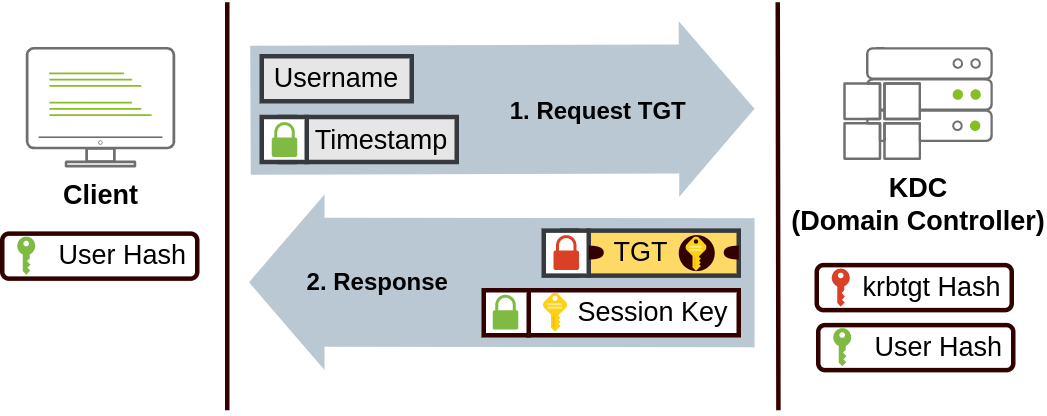
\includegraphics[scale=0.35]{Complete_Beginner_Path/Windows_Exploitation_Basics_Room/AD_Authentication_1.png}\\
To further access services, the user uses a different ticket, namely a \textbf{Ticket Granting Service (TGS)} to connect to the service they were created for in the following way:
\begin{enumerate}[resume]
\item The user sends their username along with a timestamp encrypted using the Session Key, the TGT and a \textbf{Service Principal Name (SPN)} indicating the requested service and server names. 
\item The Kerberos Distribution Center responds with the TGS encrypted using a key derived from the \textbf{Service Owner Hash}, i.e a hash known to the Service Owner, the machine the desired service runs under, and the \textbf{Service Session Key} to authenticate to the desired service.
\item The user sends the TGS to the service to authenticate and establish a connection.
\item The Service Owner accesses and validates the Service Session Key by decrypting the TGS using its configured account's password hash.
\end{enumerate}
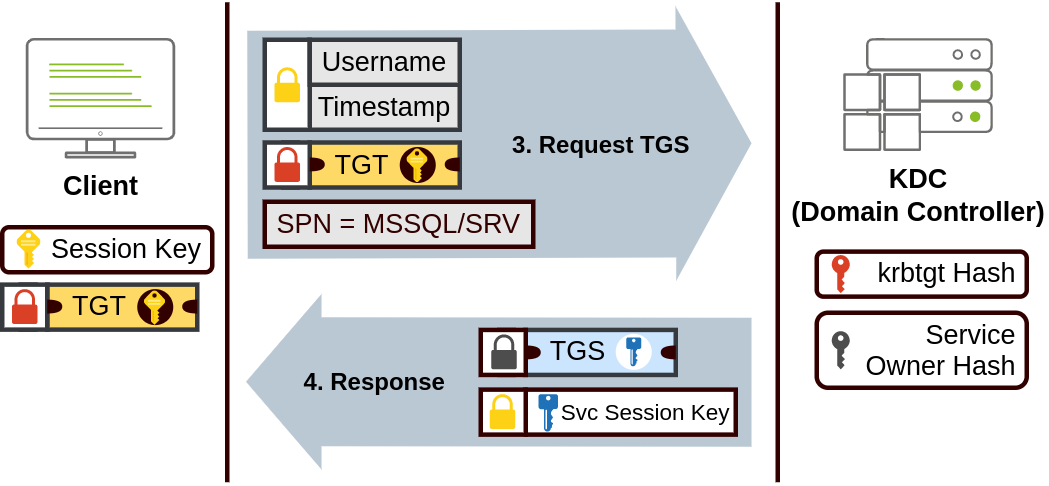
\includegraphics[scale=0.35]{Complete_Beginner_Path/Windows_Exploitation_Basics_Room/AD_Authentication_2.png}\\
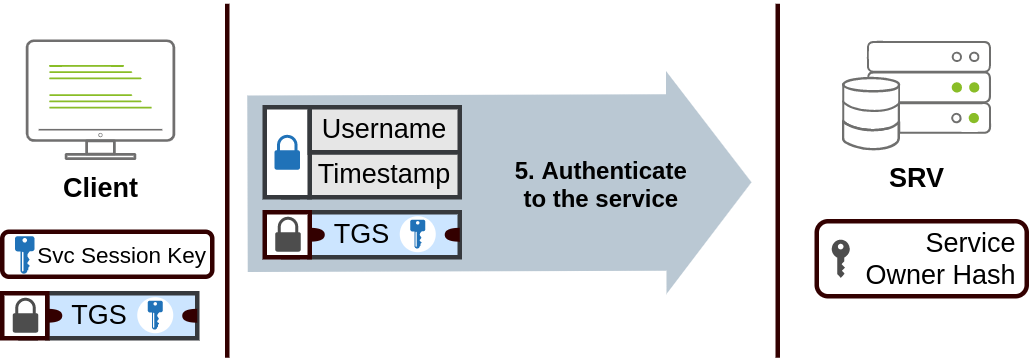
\includegraphics[scale=0.35]{Complete_Beginner_Path/Windows_Exploitation_Basics_Room/AD_Authentication_3.png}\\

On the other hand, NetNTLM works with a challenge response mechanism in the following way:\\
\begin{enumerate}
\item The client sends the server an authentication request.
\item The server answers with an NTLM challenge consisting of a random number.
\item The client responds with a message consisting of a hash made of the server challenge and their private NTLM password hash, together with some other data.
\item The server forwards this response together with its own challenge to the Domain Controller. 
\item The DC re-generates a response to the challenge posed by the server and compares it to the response generated by the client. \\
A match authenticates the client, a mismatch denies authentication.
\item This authentication response is sent back to the server.
\item The server forwards the authentication response to the client. 
\end{enumerate}
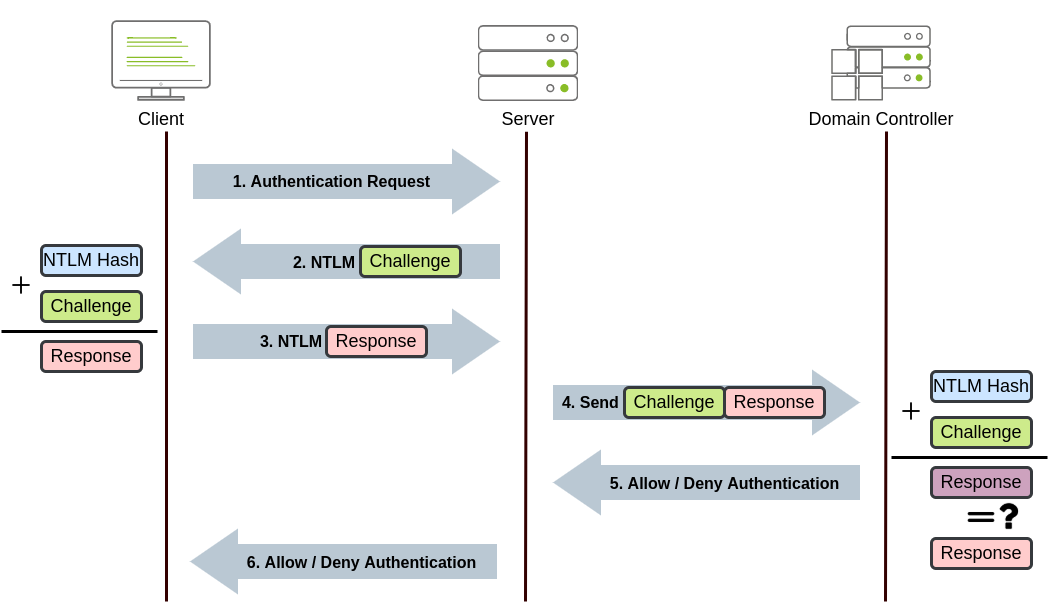
\includegraphics[scale=0.35]{Complete_Beginner_Path/Windows_Exploitation_Basics_Room/AD_Authentication_4.png}\\
Note that the NTLM password is only transmitted as a hash, never in plaintext.\\
This process only takes place when accessing a domain account, as local authentication can be verified within the server itself by comparing to the hash stored in its Security Account Manager (SAM).\\

\QA{
Will a current version of Windows use NetNTLM as the preferred authentication protocol by default? (yay/nay)
}{
nay
}
\QA{
When referring to Kerberos, what type of ticket allows us to request further tickets known as TGS?
}{
The question asks for the allowing ticket, not for the acronym TGS itself.\\
The ticket allowing a user to ask for further TGS tickets is the \textbf{Ticket Granting Ticket} TGT
}
\QA{
When using NetNTLM, is a user's password transmitted over the network at any point? (yay/nay)
}{
nay
}
}
\T{Trees, Forests and Trusts}{
After discussing the functioning of a single domain in the previous tasks, we will now deal with the relations between multiple domains.\\
This might be needed in case of different legislative frameworks, e.g when administering servers across multiple countries, or when coordinating different teams with rights over their corresponding areas which need to be encapsulated from the other servers.\\
One can always have a larger OU structure and rely on delegations, but its tendence to human errors makes it more desirable to partition the network into manageable units.\\
This partition off the network is supported natively by Active Directory, which then allows for a re-integration of those equally called domains into a tree as subdomains of the root domain, e.g adding a regional or country prefix such as \cd{de.thm.local}.\\
This allows for a partition of each subdomain independently, but introduces a security group of ``super users'', the \textbf{Enterprise Admins}. Users in this OU have admin privileges over all domains in the tree. Note that this does not revert the privileges of each subdomain's Domain Admins.\\
A union of trees corresponding to e.g a merging of enterprises is called a forest.\\

In case this encapsulation and organisation into forests and trees ever becomes too ``tight'' in its encapsulation, e.g regarding file sharing or file access, one can resort to \textbf{Trust Relationships}.\\
These Trust Relationships allow for a user in a (sub)domain access resources form another (sub)domain located in another tree of the forest, if necessary. One says that a domain trusts another if every user of the second domain can be authorised to access resources of the first domain. This does not imply automatic access authorisation, which has to be granted by the administration, only its eventual possibility.\\
These trust relationships can be one- or two-way relationships depending on the reciprocity of the trust.
\QA{
What is a group of Windows domains that share the same namespace called?
}{
Tree
}
\QA{
What should be configured between two domains for a user in Domain A to access a resource in Domain B?
}{
A Trust Relationship
}

}